\documentclass[12pt]{article}
%\usepackage[T1]{fontenc}
\usepackage{cite}
\usepackage[letterpaper,left=1in,right=1in,top=1in,bottom=1in]{geometry}
\setlength{\parindent}{15pt} % Default is 15pt.
\usepackage{setspace}
\usepackage{courier}
\usepackage{enumitem}
\usepackage{amsmath}
\usepackage{graphicx}
\usepackage{placeins}
%\onehalfspacing
\usepackage{color}

\pretolerance=10000
\tolerance=2000 
\emergencystretch=10pt

\usepackage{listings}
\definecolor{mygreen}{rgb}{0,0.6,0}
\definecolor{mygray}{rgb}{0.5,0.5,0.5}
\definecolor{mymauve}{rgb}{0.58,0,0.82}

\lstset{ %
	backgroundcolor=\color{white},   % choose the background color; you must add \usepackage{color} or \usepackage{xcolor}
	basicstyle=\scriptsize,        % the size of the fonts that are used for the code
	breakatwhitespace=false,         % sets if automatic breaks should only happen at whitespace
	breaklines=true,                 % sets automatic line breaking
	captionpos=b,                    % sets the caption-position to bottom
	commentstyle=\color{mygreen},    % comment style
	deletekeywords={...},            % if you want to delete keywords from the given language
	escapeinside={\%*}{*)},          % if you want to add LaTeX within your code
	extendedchars=true,              % lets you use non-ASCII characters; for 8-bits encodings only, does not work with UTF-8
	frame=single,                    % adds a frame around the code
	keepspaces=true,                 % keeps spaces in text, useful for keeping indentation of code (possibly needs columns=flexible)
	keywordstyle=\color{blue},       % keyword style
	language=Octave,                 % the language of the code
	morekeywords={*,...},            % if you want to add more keywords to the set
	numbers=left,                    % where to put the line-numbers; possible values are (none, left, right)
	numbersep=5pt,                   % how far the line-numbers are from the code
	numberstyle=\tiny\color{mygray}, % the style that is used for the line-numbers
	rulecolor=\color{black},         % if not set, the frame-color may be changed on line-breaks within not-black text (e.g. comments (green here))
	showspaces=false,                % show spaces everywhere adding particular underscores; it overrides 'showstringspaces'
	showstringspaces=false,          % underline spaces within strings only
	showtabs=false,                  % show tabs within strings adding particular underscores
	stepnumber=2,                    % the step between two line-numbers. If it's 1, each line will be numbered
	stringstyle=\color{mymauve},     % string literal style
	tabsize=2,                       % sets default tabsize to 2 spaces
}

\begin{document}
	
	\title{CS 5220: Homework 2}
	\date{\today}
	\author{Group 19: Robert Carson (rac428), Robert Chiodi (rmc298), Sam Tung (sat83)}
	\maketitle
		
	\section{Initial Profiling}
	In order to perform initial profiling of the code before any improvements are made, Intel's VTUNE was used via the terminal command line on Totient. In an attempt to get the most accurate results (taken with a large sample size), we decided to gather data while running the large wave simulation, invoked with the command \texttt{make big}. Information collected from VTUNE's ``advanced-hotspots'' option is used in our analysis.
		\subsection{Whole Program - Advanced Hotspots}
		First, hotspots in the entire program were examined in order to determine where our efforts should be directed. The time taken in the top 10 most time consuming functions can be seen below in Figure~\ref{top10}. Of these, it is clear that most of our optimization efforts should be directed to the functions \texttt{limited\_derivs}, \texttt{compute\_step}, and \texttt{compute\_fg\_speeds}. These functions were then examined individually, once again using VTUNE on our advanced-hotspots collection.
		\begin{figure}[h!]
			\begin{center}
				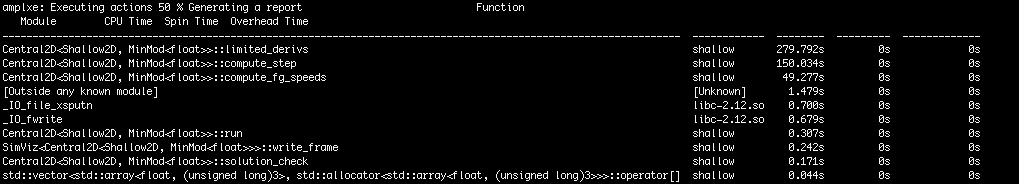
\includegraphics[width=0.7\columnwidth]{top10}
				\caption{Top 10 most time consuming functions in the wave simulation. Generated using Intel's VTUNE on Totient.}
				\label{top10}
			\end{center}
		\end{figure}
		\subsection{\texttt{limited\_derivs} - Advanced Hotspots}
		The function \texttt{limited\_deriv} is used to calculate the fluxes into and out of each cell in order to advance to the next time step. This involves a three point computational stencil in each direction and loops through the entire domain interior (the whole domain except for those where boundary conditions are applied). Each point requires $\mathtt{du.size()}\times 9$ floating point operations as well as $\mathtt{du.size()} \times 2$ calls to the intrinsic function $\mathtt{min}$. Sadly, the hotspot analysis on the \texttt{limited\_deriv} function, shown in Figure~\ref{init_lim_deriv}, does not give any hints on possible optimizations or bottle necks.
		
		\begin{figure}[h!]
			\begin{center}
				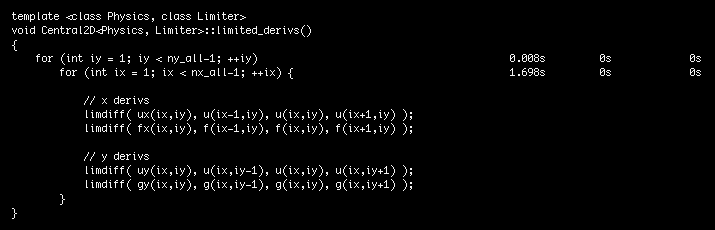
\includegraphics[width=0.7\columnwidth]{init_lim_deriv}
				\caption{Time taken to perform each loop present in \texttt{limited\_derivs}, recorded in core-seconds.}
				\label{init_lim_deriv}
			\end{center}
		\end{figure}
		
		\subsection{\texttt{compute\_step} - Advanced Hotspots}
		The purpose of \texttt{compute\_step} is to update the wave equation to the next time step using a predictor-corrector method. First, the fluxes are calculated in the prediction. Next, the corrector step uses the predicted fluxes, the differences in velocities, and the current velocities, to advance to the next time state. Luckily, VTUNE's report is more helpful than in the previous case, and provides extensive timings for this function, shown in Figure~\ref{init_compute_step}. The calculation in the corrector step can be seen as the most expensive cost of the function. It is important to note, however, that the predictor step and copying of the solution to the \texttt{u} array sum to half of the function's cost.
		\begin{figure}[h!]
			\begin{center}
				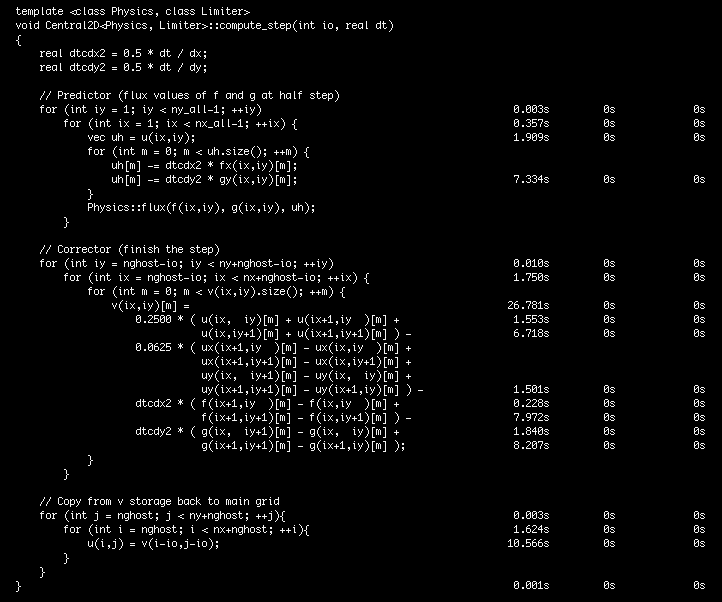
\includegraphics[width=0.7\columnwidth]{init_compute_step}
				\caption{Time taken to perform each loop present in \texttt{compute\_step}, recorded in core-seconds.}
				\label{init_compute_step}
			\end{center}
		\end{figure}	
		
		\subsection{\texttt{compute\_fg\_speeds} - Advanced Hotspots}
		The function of \texttt{compute\_fg\_speeds} has two primary responsibilities: to update the cell centered fluxes, \texttt{f} and \texttt{g}, and to calculate the maximum speed in the domain, allowing dynamic adjustment of the time step in order to satisfy the CFL condition and ensure numerical stability. The timing data for this function can be seen in Figure~\ref{init_compute_fg_speeds}. While the most time consuming portion of the code is most likely the calculation of the fluxes and wave speed (both of which are in the \texttt{Shallow2d} structure), the calls to the intrinsic function \texttt{max} also represent a non-trivial amount of time. 	
		\begin{figure}[h]
			\begin{center}
				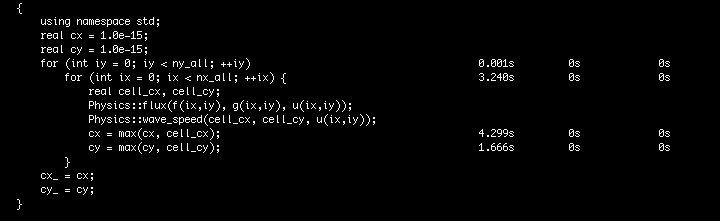
\includegraphics[width=0.7\columnwidth]{init_compute_fg_speeds}
				\caption{Time taken to perform each loop present in \texttt{compute\_fg\_speeds}, recorded in core-seconds.}
				\label{init_compute_fg_speeds}
			\end{center}
		\end{figure}	
		
		\FloatBarrier
	\section{Parallelization}
	While we are aware that the optimal programming of this code will not wholly be due to parallelization by OpenMP, it is most certainly necessary. Furthermore, future tuning and optimization of the code may change depending on whether the code is run in serial or parallel. For these reasons, we first decided to parallelize the code and compare its performance against the initial, serial code.
		\subsection{Naive Implementation of OpenMP}
		First, a naive implementation of OpenMP using pragmas was used. This involved placing \texttt{\#pragma omp parallel for} in front of the start of each for loop in the functions \texttt{init}, \texttt{apply\_periodic}, \texttt{compute\_fg\_speeds}, \texttt{limited\_derivs}, and \texttt{compute\_step}. This proved to improve performance significantly when run on one node of Totient (24 threads), as seen in Figure~\ref{naive_omp}. It should be noted that the time shown is the total processor time spent and not the per processor time.
		
%		! Will include rest of part on how it performed better. Need to run 'big' simulation.
		
		\begin{figure}[h]
			\begin{center}
				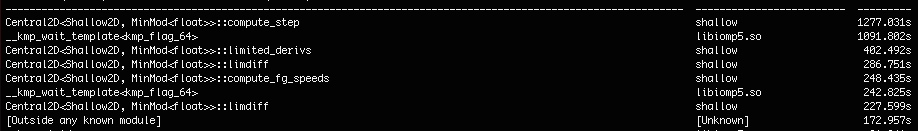
\includegraphics[width=0.7\columnwidth]{naive_omp}
				\caption{Timing of entire simulation using naive implementation of OpenMP parallelized for-loops. Generated using Intel's VTUNE on Totient and recorded in core-seconds.}
				\label{naive_omp}
			\end{center}
		\end{figure}
		
		\subsection{OpenMP for with \texttt{collapse}}
		``OpenMP parallel for'' also has the \texttt{collapse} option, which essentially informs OpenMP how many nested loops are present. By knowing this, OpenMP is able to section both loops to run on multiple processors, creating blocks for each processor to work on. Results when using \texttt{collapse} can be seen in Figure ~\ref{collapse_omp}. It should be noted that the time shown is the total processor time spent and not the per processor time. It was found that using the \texttt{collapse} option actually led to worse performance. We believe this is due to the creation of blocks, which will limit the amount of memory accesses each core has that is of unit stride. When only sectioning the for loops based on the vertical (y) direction, each processor gets a $n \times nx$ block of the array, where $n$ is some number of rows (vertical lines of computational cells) in the domain. This increases memory access locality, which in turn increases cache hits.
			
%		! Will include rest of part on how it performed worse. Need to run 'big' simulation.
			
		\begin{figure}[h]
			\begin{center}
				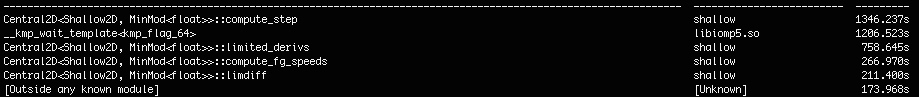
\includegraphics[width=0.7\columnwidth]{collapse_omp}
				\caption{Timing of entire simulation using implementation of OpenMP parallelized for-loops with \texttt{collapse} option. Generated using Intel's VTUNE on Totient and recorded in core-seconds.}
				\label{collapse_omp}
			\end{center}
		\end{figure}
		
		\subsection{OpenMP thread creation limited:}
		
		The constant creation of threads creates a large overhead cost that negatively affects the performance of the program. Therefore, the fewer times that a pool of threads needs to be created the better. In the previous examples, the thread pools were created each time a parallel for loop was called. In order to reduce this costly operation, a pool of threads was only  created within the main run function as shown in the below code section.
		
		\begin{verbatim}
	    for (int io = 0; io < 2; ++io) {
            real cx, cy;
            #pragma omp parallel
            {
            apply_periodic();
            compute_fg_speeds(cx, cy);
            limited_derivs();
            #pragma omp single
                {
            if (io == 0) {
                dt = cfl / std::max(cx/dx, cy/dy);
                if (t + 2*dt >= tfinal) {
                    dt = (tfinal-t)/2;
                    done = true;
                }
            }
                }
            compute_step(io, dt);
            #pragma omp single
            t += dt;
            }

		\end{verbatim}
		
		\noindent Sections of the code that only required one thread to execute took advantage of the omp single pragma command which tells only one thread to run that section of code while the rest wait for it to finish. Inside each of the computation calls the regular omp for pragma command is used to parallelize the various for loops being run. The performance of this operation for the top five costliest function calls when run on the big simulation can be found in Figure ~\ref{ThreadMovement}.
		
		\begin{figure}[h!]
			\begin{center}
				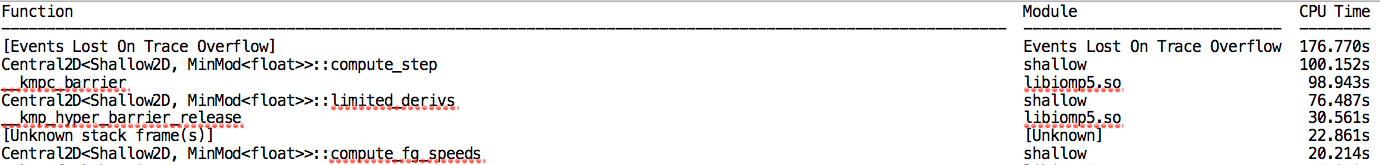
\includegraphics[width=0.8\columnwidth]{ThreadMovement}
				\caption{Timing of five costliest functions using fewer thread creation events. Generated using Intel's VTUNE on Totient.}
				\label{ThreadMovement}
			\end{center}
		\end{figure}
		
		\noindent It should also be noted that these results do include the effects of attempting to force the compiler to vectorize several loops by replacing the min and max calls with an equivalent if statement min and max code. Also from Figure ~\ref{ThreadMovement}, it can be seen that the program still spends a large amount of time in block operations. Based on Figure ~\ref{naive_omp}, it appears that the main cost of thread creation is no longer one of the top performance issues with the code. Now, the internal barrier times is of much more concern.
		
		\subsection{OpenMP nowait implementation:}
		When using the \texttt{omp for} pragma command, an implicit barrier is placed at the end of the loops. Due to the nature of this program, it is possible in several places to be able to assume that a barrier is not needed, and therefore the \texttt{nowait} pragma command can be used. The nowait command could be safely used in the \texttt{compute\_fg\_speeds} and \texttt{limited\_derivs} functions. Then it could be partially used in the \texttt{compute\_step} function once the predictor step was calculated. If the nowait command was used for the predictor loop, synchronization issues are possible when a thread is able to go onto the corrector step while other threads are still in the predictor step. The performance of this implementation for the top five costliest function calls when run on the ``big'' simulation can be found in Figure~\ref{bindoff}
		
		\begin{figure}[h]
			\begin{center}
				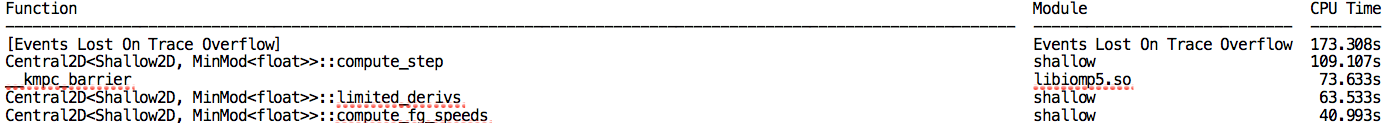
\includegraphics[width=0.8\columnwidth]{bindoff}
				\caption{Timing of five costliest functions using \texttt{nowait} pragma command. Generated using Intel's VTUNE on Totient.}
				\label{bindoff}
			\end{center}
		\end{figure}
		
		\noindent It can be seen by comparing Figure~\ref{ThreadMovement} and Figure~\ref{bindoff} that the overall time spent in the barrier function call has gone down drastically by including the nowait call.
		
		\subsection{Thread Affinity:}
		OpenMP 4.0 offers the ability to describe the ordering of the threads among the CPUs/MICs. Threads can be placed near each other on the same CPU using the OpenMP pragma command \texttt{proc\_bind(close)}. The benefit of doing this is that amount of time for synchronization between threads should decrease. The downside of this is that the available cache and bandwidth per thread will decrease. Another option available distributes the threads more evenly throughout the available CPUs/MIC, and it can be turned on using the OpenMP pragma command \texttt{proc\_bind(spread)}. It should lead to the opposite effects of the close command. The thread affinity was implemented on the code base that used the \texttt{nowait} pragma command. The performance of this implementation for the top five costliest function calls when run on the big simulation can be found in Figure ~\ref{nowait} and Figure ~\ref{nowait2} for the \texttt{proc\_bind(close)} pragma command. Due to system traffic, timing can vary across multiple runs. For this reason, two figures were shown so some measure of variance could be judged. The results for the \texttt{proc\_bind(spread)} command can be found in Figure ~\ref{bindspread}.
		
		\begin{figure}[h]
			\begin{center}
				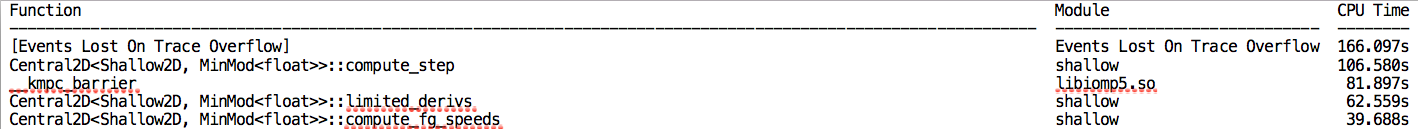
\includegraphics[width=0.8\columnwidth]{nowait}
				\caption{Timing of five costliest functions using \texttt{proc\_bind(close)} pragma command for run 1. Generated using Intel's VTUNE on Totient.}
				\label{nowait}
			\end{center}
		\end{figure}
		
		\begin{figure}[h]
			\begin{center}
				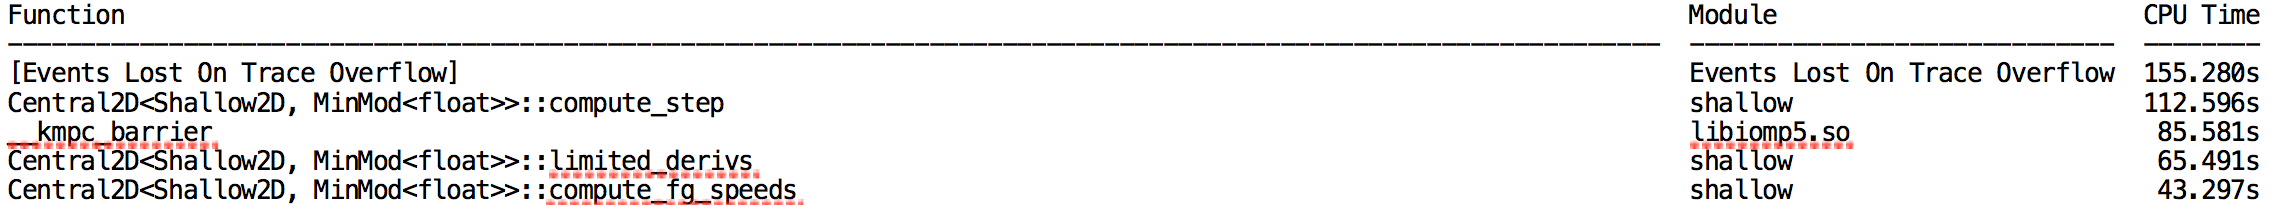
\includegraphics[width=0.8\columnwidth]{nowait2}
				\caption{Timing of five costliest functions using \texttt{proc\_bind(close)} pragma command for run 2. Generated using Intel's VTUNE on Totient.}
				\label{nowait2}
			\end{center}
		\end{figure}
		
		\begin{figure}[h]
			\begin{center}
				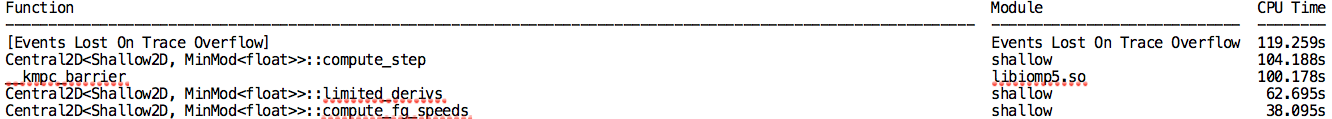
\includegraphics[width=0.8\columnwidth]{bindspread}
				\caption{Timing of five costliest functions using \texttt{proc\_bind(spread)} pragma command. Generated using Intel's VTUNE on Totient.}
				\label{bindspread}
			\end{center}
		\end{figure}
		
		\noindent Overall, both thread affinity options have shown to lead to decreased performance. Therefore, they will not be used in the production code.
		
\section{Analysis}
The current implementation, while offering a sizable speed up over the strictly serial version, still leads much to be desired. Since it currently depends on the \texttt{parallel for} command to run with OpenMP automating certain commands, barriers are automatically placed into the code that limits how each processor accesses the memory of the variables. Further improvements can be made to the code by eliminating these blocking structures where allowed and only syncing the data when the need arises in order to reduce the amount of overhead costs that occur from this type of synchronization. One such place where this could be beneficial is in the \texttt{compute\_step} function. Specific structures could be used in order to ensure the predictor step is done for edge cases before the corrector loop begins without requiring a barrier. To do this, a more rigorous implementation of OpenMP will need to be done, which mimics more of a distributed memory parallel code. Blocks will be made of the domain, where each subdomain has ghost cells and is unaware of what happens outside of itself (except through the ghost cells). This gives more control and limits necessary communication.

\subsection{Strong and Weak Scaling}
The current version of the code can be analyzed for its strong and weak scaling capabilities. The strong scaling will be tested using the ``big'' wave test case with 1000 points in each direction and 100 time steps between frames. The results can be seen in Table~\ref{sstable}. This is tested on the main Xeon chips. With the highest number of threads tested being 16, inter-node communication costs were avoided. VTUNE analysis was also not collected in order to remove any additional time the collection process takes. In Table~\ref{strongscale}, strong scaling is defined by Eq.~\ref{strongscale} and strong scaling efficiency is defined by Eq.~\ref{normss}.

\begin{equation}
\mathrm{Strong \; Scaling} = \frac{t_{\mathrm{serial}}}{t_{\mathrm{parallel}}}
\label{strongscale}
\end{equation}

\begin{equation}
\mathrm{Strong \; Scaling \; Efficiency} = \frac{t_{\mathrm{serial}}}{t_{\mathrm{parallel}}} \frac{1}{p}
\label{normss}
\end{equation}
where $t_{\mathrm{serial}}$ and $t_{\mathrm{parallel}}$ are the times taken when running in serial or parallel, respectively, and $p$ is the number of processors. The strong scaling efficiency is essentially what percentage of perfect linear scaling is actually achieved. This is plotted in Figure~\ref{ssplot}.

\begin{table}[h]
	\begin{center}
		\begin{tabular}{|c c c c|}
			\hline
			Threads & Total Time (seconds) & Strong Scaling & Strong Scaling Efficiency \\ \hline
			1 & 539 & 1.0  & 100\% \\ \hline
			2 & 288 & 1.87 &  93.5\% \\ \hline
			4 & 218 &  2.47&  61.7\%  \\ \hline
			8 & 198 &  2.72&  34.0\%  \\ \hline
			16 & 188 &  2.87& 17.9\%   \\ \hline
		\end{tabular}
		\caption{Strong scaling for wave simulation with 1000 mesh points in each direction and 100 timesteps between frames.}
		\label{sstable}
	\end{center}
\end{table}

		\begin{figure}[h]
			\begin{center}
				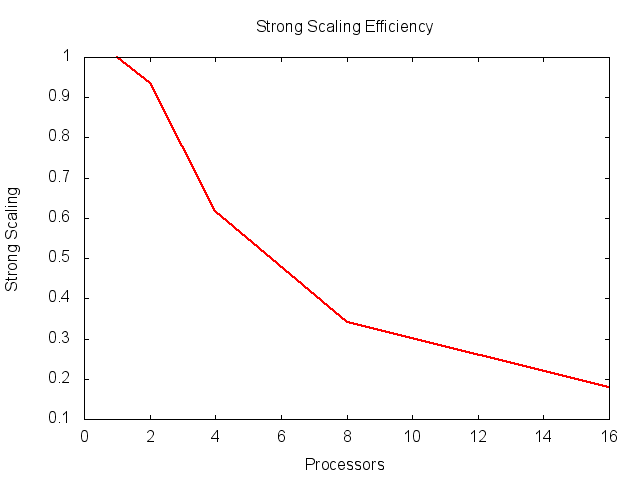
\includegraphics[width=0.5\columnwidth]{ssplot}
				\caption{Plot of strong scaling, representing the data shown in Table~\ref{sstable}.}
				\label{ssplot}
			\end{center}
		\end{figure}

For weak scaling, three simulations were performed, scaling the number of processors equally with the number of cells. The results can be seen in Table~\ref{wstable}. Here, weak scaling is defined by Eq.~\ref{ws}. It was decided to double the side length for each simulation in order to perform the weak scaling test, meaning the number of processors needed to be quadrupled for each run. A plot of the weak scaling can also be seen in Figure~\ref{wsplot}. A more thorough weak scaling test is planned for the future.

\begin{equation}
\mathrm{Weak \; Scaling} = \frac{t_{\mathrm{serial}}(n(p))}{t_{\mathrm{parallel}}(n(p),p)}
\label{ws}
\end{equation}

\begin{table}[h]
	\begin{center}
		\begin{tabular}{|c c c c|}
			\hline
			Threads & Cells Per Side & Total Time (seconds) & Weak Scaling \\ \hline
			1 & 200 & 4.0 & 1.00   \\ \hline
			4 & 400 & 8.3 & 0.485 \\ \hline
			16 & 800 & 73.5 & 0.0544   \\ \hline
		\end{tabular}
		\caption{Strong scaling for wave simulation with 1000 mesh points in each direction and 100 timesteps between frames.}
		\label{wstable}
	\end{center}
\end{table}

		\begin{figure}[h]
			\begin{center}
				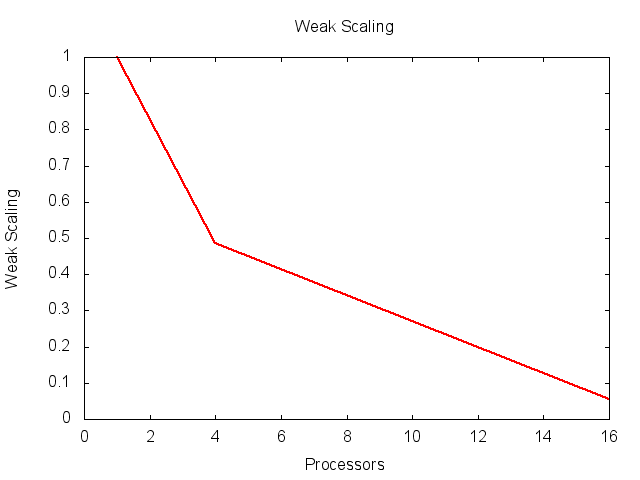
\includegraphics[width=0.5\columnwidth]{wsplot}
				\caption{Plot of weak scaling, representing the data shown in Table~\ref{wstable}.}
				\label{wsplot}
			\end{center}
		\end{figure}

We believe the weak scaling performance is very poor due to our implementation of OpenMP. Weak scaling usually tests the importance of communication on distributed memory systems, since each processor should be performing the same amount of algorithmic work as it is in the serial case. The main difference is the size of data being communicated is largely increased with the scaling in problem size. Since this is a shared memory code, we believe this indicates poor memory handling, leading to many cache misses. This is especially evident in the largest case, where we believe the problem size exceeded the cache size, causes very poor memory use. This could be fixed by a blocking scheme, where the domain is decomposed into subdomains, in order to increase memory locality, reducing the number of cache misses substantially. Another possible reason for the poor performance of the 16 thread case is an increase in time for each communication, due to the threads existing on two separate chips.

The scaling can be represented theoretically by creating an equation for the parallel time taken in the code. This would be primarily made up of two parts: the time to perform the floating point operations, and the portion spent communicating and synchronizing. In this code, since it uses shared memory, the only communications required involves OpenMP barriers and informing each processor of their section of the ``for loops''. These communications will be incorporated into the relation using the variable $t_c$. Predicting the value of $t_c$ consistently is difficult due to uncertainty in how long processors will be required to wait at a barrier. Through running simulations with various parameters, it may be possible to get a rough estimate of the communication time per processor, which could then be used in this model to approximate the scaling for a specific simulation. 

The expression for time taken to execute the simulation in parallel can be represented by Eq.~\ref{part}.

\begin{equation}
t_{\mathrm{parallel}} = \frac{t_{\mathrm{serial}}}{p} + p t_c
\label{part}
\end{equation}

This equation assumes that the serial work will be evenly distributed among all processors, leading to the serial work being completed in $t_{\mathrm{serial}}/p$ time. The cost of parallelizing the code per processor, in the form of communication, barriers, and synchronization, is represented by $t_c$. With an expression for the parallel time, it is now possible to create a rough approximation for scaling, shown in Eq.~\ref{exps}. The difference in strong and weak scaling appears in the values used for $t_{\mathrm{serial}}$ and $t_c$.

\begin{equation}
\mathrm{Scaling} \approx \frac{t_{\mathrm{serial}}}{t_{\mathrm{parallel}}} = \frac{t_{\mathrm{serial}}}{\frac{t_{\mathrm{serial}}}{p} + p t_c} = \left (\frac{1}{p}+p \frac{t_c}{t_{\mathrm{serial}}} \right)^{-1}
\label{exps}
\end{equation}

\section{Future Work}
Once the code has been parallelized with subdomains using OpenMP, use of the Xeon Phi chips will be implemented in the code. Thus far, we have had trouble using the Xeon Phi chips via the \texttt{\#pragma offload target (mic:0)} command. We are not entirely sure of the issue, but believe it has to do with the use of templates in the C++ version of the code.

Once the code is parallelized into subdomains and effectively offloaded to the Xeon Phi chip, we will attempt to vectorize the loops. Preliminarily, we have had trouble vectorizing the loops within the C++ memory structure currently used, and have not managed to use the \texttt{restrict} keyword. Without this, the compiler is easily confused about dependencies inside the loop, as it cannot be sure where separate pointers are pointing to. It may be necessary to switch to the C version of the code that was written by Professor Bindel in order to tune the code for better vectorization.


%\FloatBarrier
%	\bibliography{report.bib} 
%	\bibliographystyle{unsrt}
	
\end{document}